\documentclass[fontsize=8pt, a4paper, landscape, fleqn]{scrartcl}

\usepackage[utf8]{inputenc}
\usepackage[english]{babel}
%\usepackage[standardsections]{scrhack}
%\usepackage[raggedright]{titlesec} %% Gibt warnings
\usepackage{xcolor, sectsty}
\usepackage{enumerate, enumitem, ulem, graphicx, multirow, comment}
\usepackage{listings}
\usepackage{wrapfig} 
\usepackage{titlesec}     % For customizing section titles
\usepackage{twemojis}     % Für Emojis

%Graph
\usepackage{tikz}
\usetikzlibrary{positioning}
\usetikzlibrary{trees}
\usepackage{pgfplots}

%Page reference
\usepackage{hyperref}
\usepackage{xparse,nameref}
\hypersetup{
pdfborder={0 0 0}, % Add this line to remove the link border
}

%code layout
\definecolor{sec}{RGB}{40,56,71}
\definecolor{subsec}{RGB}{72,98,124}
\definecolor{subsubsec}{RGB}{102,141,178}
\definecolor{codegreen}{rgb}{0,0.6,0}
\definecolor{codegray}{rgb}{0.5,0.5,0.5}
\definecolor{codepurple}{rgb}{0.58,0,0.82}
\definecolor{backcolour}{RGB}{240,240,240}
\usepackage{tcolorbox}
\tcbuselibrary{minted, breakable}

% Define custom colors
\definecolor{sectioncolor}{RGB}{64, 64, 64}       % Dark Gray
\definecolor{subsectioncolor}{RGB}{70, 130, 180}  % Steel Blue

% Custom section and subsection commands with unified styling
\renewcommand{\section}[1]{%
    \noindent\colorbox{sectioncolor}{%
        \parbox{\dimexpr\columnwidth-2\fboxsep}{\color{white}\textbf{#1}}}%
    \vspace{0.5mm}% Optional spacing after the section
}

\renewcommand{\subsection}[1]{%
    \noindent\colorbox{subsectioncolor}{%
        \parbox{\dimexpr\columnwidth-2\fboxsep}{\color{white}\textbf{#1}}}%
    \vspace{0.5mm}% Optional spacing after the subsection
}

% Optional: Customize subsubsection or other title levels
\renewcommand{\subsubsection}[1]{%
    \noindent\textbf{\textit{\color{subsectioncolor}#1}}% Italic with subsection color
    \vspace{1mm}% Optional spacing after subsubsection
}
%Layout
\usepackage{multicol, geometry, titlesec, xcolor}
\geometry{margin=0.2cm}
%\titlespacing{\section}{0pt}{3pt}{1pt}
%\titlespacing{\subsection}{0pt}{3pt}{1pt}
%\titlespacing{\subsubsection}{0pt}{3pt}{1pt}
\parindent 0pt

%Remove numbering
\pagestyle{empty} 
%\pagenumbering{arabic}

\setlist[itemize]{leftmargin=2mm, itemsep=0mm} %{nosep}
\setlist[enumerate]{leftmargin=3mm, nosep} %{nosep}

\newlength{\breite}
\setlength{\breite}{0.5pt}
\setlength{\columnseprule}{\breite}

\usepackage{graphicx}

%Style code
\usepackage{minted}
\lstdefinestyle{mystyle}{
    backgroundcolor=\color{backcolour},
    commentstyle=\color{codegreen},
    keywordstyle=\color{blue},
    numberstyle=\tiny\color{codegray},
    stringstyle=\color{codepurple},
    basicstyle=\ttfamily,
    breakatwhitespace=false,
    breaklines=true,
    captionpos=b,
    keepspaces=true,
%    numbers=left,
    numbersep=5pt,
    showspaces=false,
    showstringspaces=false,
    showtabs=false,
    tabsize=2,
}
\lstset{style=mystyle}

%Mathematics
\usepackage{amsmath, amstext, amssymb, mathtools, esint, polynom}
\allowdisplaybreaks 

%Document file
\begin{document}
\begin{multicols*}{3}[\raggedcolumns]
\section{Introduction to the Climate System}
\subsection{Climate Definition}
\begin{itemize}
    \item The synthesis of weather in a particular region.
    \item Defined by Expected Values of meteorological elements such as:
    \begin{itemize}
        \item Temperature \twemoji{thermometer}
        \item Precipitation \twemoji{umbrella}/\twemoji{snowflake}
        \item Wind
        \item Pressure \twemoji{bomb}
        \item Cloudiness \twemoji{cloud}
        \item Humidity \twemoji{fog}
    \end{itemize}
\end{itemize}

\subsection{Climate Change}
\begin{itemize}
    \item 2.9°C \textit{regional} increase in Switzerland compared to preindustrial levels (1871-1900)
    \item 1.09°C (0.95-1.20) \textit{global} increase of Global surface temperature (2011–2020 vs. 1850–1900)
    \item Regional Drying
\end{itemize}

\subsection{Components of the Climate System}
\begin{wrapfigure}{r}{0.125\textwidth}
    \centering
    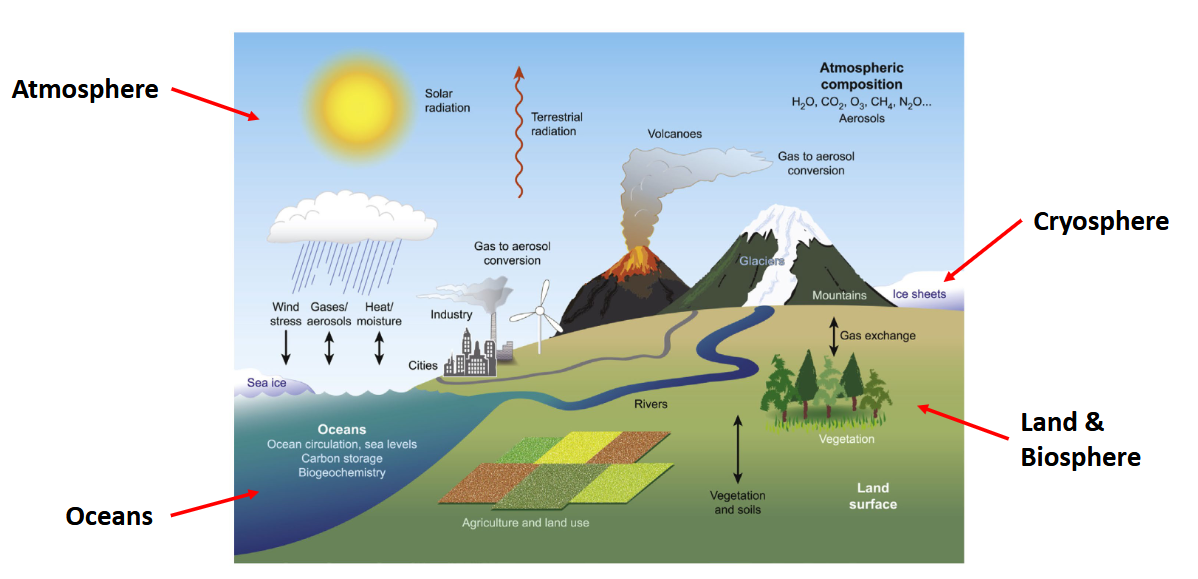
\includegraphics[width=0.12\textwidth]{Secondary/img/Pasted image 20250407144258.png}
\end{wrapfigure}
\begin{itemize}
    \item Atmosphere
    \item Ocean
    \item Cryosphere
    \item Land \& Cryosphere
\end{itemize}

\subsection{Mass Ordering of Components}
\begin{wrapfigure}{r}{0.125\textwidth}
    \centering
    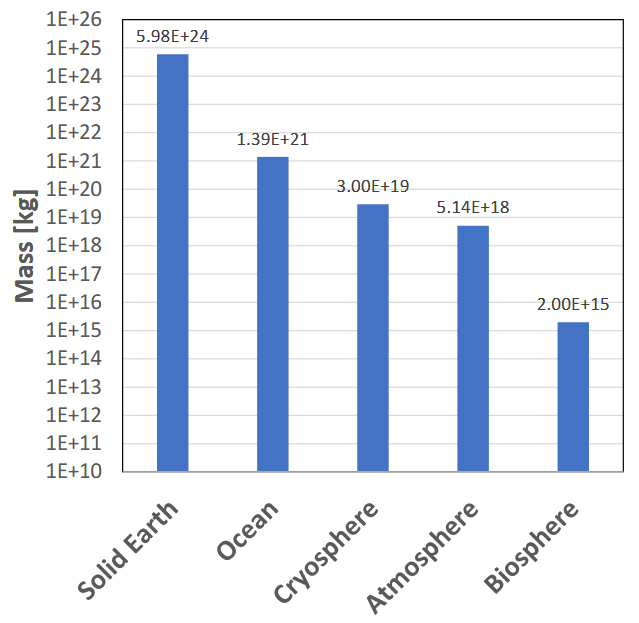
\includegraphics[width=0.12\textwidth]{Secondary/img/Pasted image 20250407160249.png}
\end{wrapfigure}
\begin{itemize}
    \item Solid Earth
    \item Ocean
    \item Cryosphere
    \item Atmosphere
    \item Biosphere
\end{itemize}

\subsection{Vertical Structure of the Atmosphere}
\begin{wrapfigure}{r}{0.125\textwidth}
    \centering
    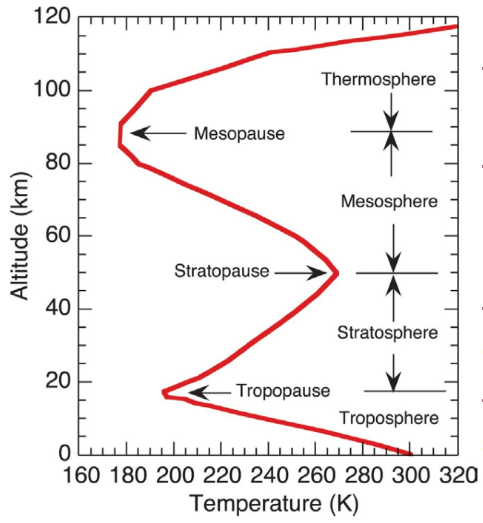
\includegraphics[width=0.12\textwidth]{Secondary/img/Pasted image 20250407145244.png}
\end{wrapfigure}
\begin{itemize}
    \item \textbf{Thermosphere} \twemoji{purple_heart}
        \begin{itemize}
            \item Temperature increases due to the absorption of solar \textit{ultraviolet} (UV) radiation
            \item Think of it as a hot layer absorbing intense sunlight! \twemoji{sun_with_face}
        \end{itemize}
    \item \textbf{Mesosphere} \twemoji{dash}
        \begin{itemize}
            \item It gets really cold up in the \textit{Mesopause}! \twemoji{cold_face}
            \item Temperature decreases as the atmosphere gets \textit{thinner}, reducing the absorption of solar radiation
        \end{itemize}
    \item \textbf{Stratosphere} \twemoji{shield}
        \begin{itemize}
            \item It's really hot up in the \textit{Stratopause}! \twemoji{hot_face}
            \item Temperature increases because \textit{Ozone} $O_3$ absorbs solar radiation 
        \end{itemize}
    \item \textbf{Troposphere} \twemoji{rainbow}
        \begin{itemize}
            \item It's quite cold in the \textit{Tropopause}! \twemoji{cold_face}
            \item Temperature decreases. Controlled by convective heating and radiative cooling.
            \item layer where we live \& where \textit{weather} happens
            \item 2 Layers: 
            \begin{wrapfigure}{r}{0.125\textwidth}
                \centering
                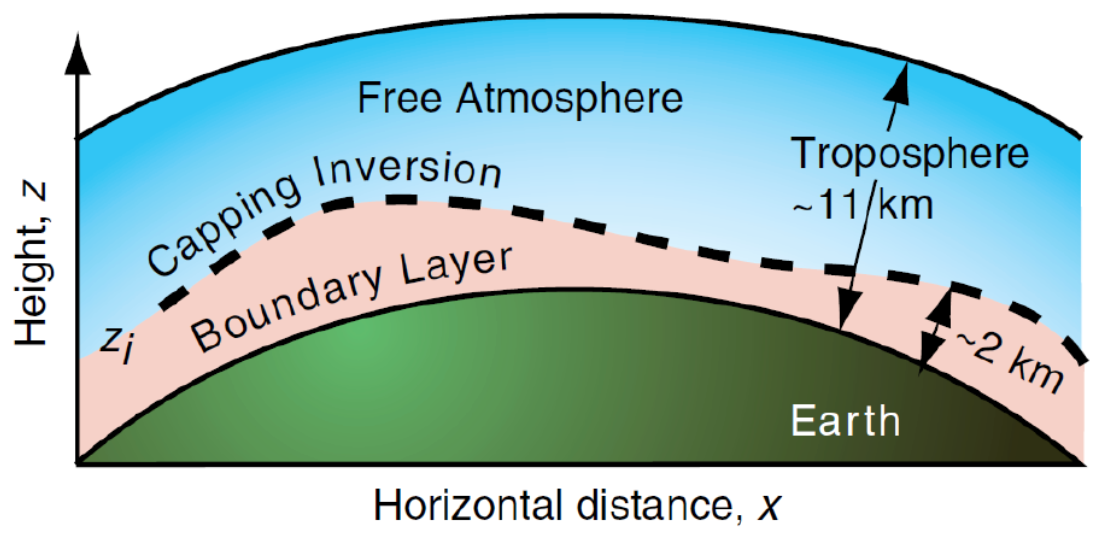
\includegraphics[width=0.12\textwidth]{Secondary/img/Pasted image 20250407155223.png}
            \end{wrapfigure}
                \begin{itemize}
                    \item 9 km Free Atmosphere
                    \item Capping Inversion Line
                    \item 2 km Boundary Layer
                \end{itemize}
        \end{itemize}
\end{itemize}

\subsection{Chemical Composition of the Atmosphere}
\begin{itemize}
    \item Main components
        \begin{itemize}
            \item Nitrogen
            \item Oxygen
        \end{itemize}
    \item Important GHGs
        \begin{itemize}
            \item Water Vapor
            \item Carbon Dioxide
            \item Methane
        \end{itemize}
\end{itemize}

\subsection{Global Energy Balance}
\begin{wrapfigure}{r}{0.125\textwidth}
    \centering
    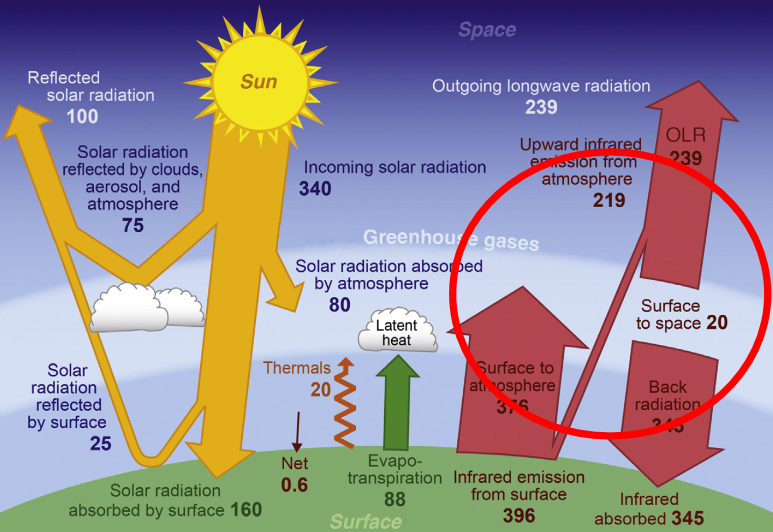
\includegraphics[width=0.12\textwidth]{Secondary/img/Pasted image 20250407170624.png}
\end{wrapfigure}

\subsection{Greenhouse Effect}
\begin{itemize}
    \item \textit{Without} the Greenhouse Effect, the mean global temperature would be \textit{33°C lower}
\end{itemize}

\subsection{Oceans}
\begin{itemize}
    \item Thermohaline Circulation 
    \begin{wrapfigure}{r}{0.125\textwidth}
        \centering
        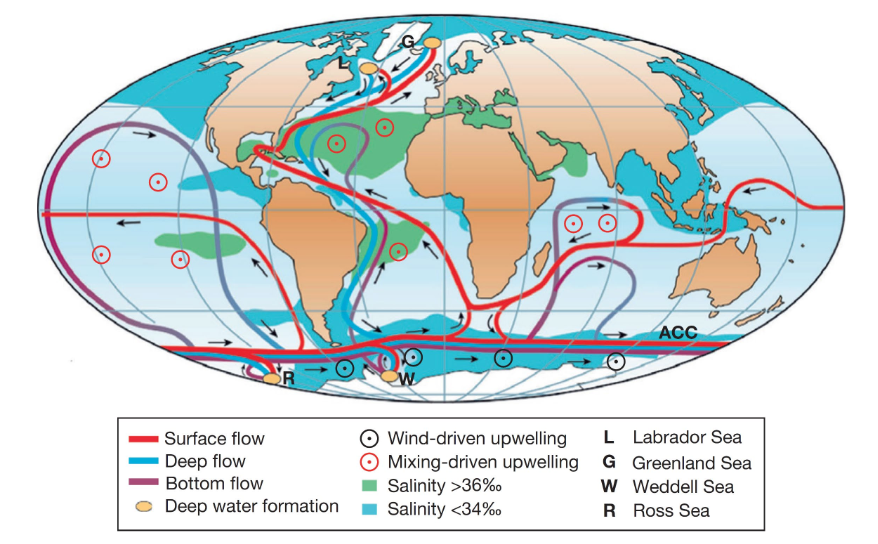
\includegraphics[width=0.1\textwidth]{Secondary/img/Pasted image 20250407171910.png}
    \end{wrapfigure}
    \item Atmosphere-Ocean Interface 
\end{itemize}

\subsection{Cryosphere}
\begin{itemize}
    \item Covers land and sea ice
    \item particularly in the Northern Hemisphere
    \item highlights rapid changes due to climate change
\end{itemize}

\subsection{Land and Biosphere}
\begin{itemize}
    \item Impact of land surface for climate:
        \begin{itemize}
            \item Spatial variations in land characteristics (Biomes)
            \item Temporal variations in land characteristics (Spring-Summer-Fall-Winter)
        \end{itemize}
    \item Human influence on land cover
    \item Vegetation in the Carbon Cycle:
    \begin{wrapfigure}{r}{0.125\textwidth}
        \centering
        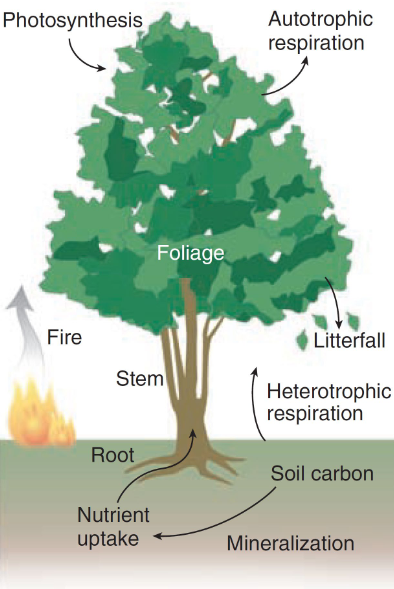
\includegraphics[width=0.1\textwidth]{Secondary/img/Pasted image 20250407172907.png}
    \end{wrapfigure}
        \begin{itemize}
            \item gross primary production (GPP) (always positive)
            \item net primary production (NPP) (always positive)
            \item net ecosystem exchange (NEE) (usually positive)
            \item net biome exchange (NBE) (positive or negative)
        \end{itemize}
\end{itemize}

\subsection{Sources \& Sinks of Global Carbon Cycle}
\begin{wrapfigure}{r}{0.125\textwidth}
    \centering
    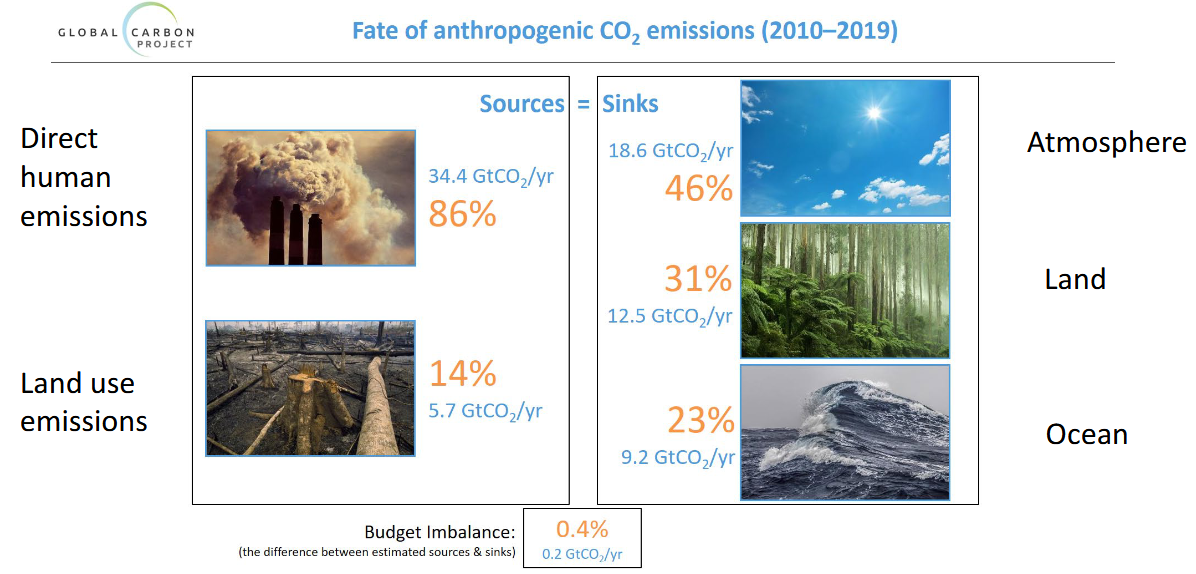
\includegraphics[width=0.12\textwidth]{Secondary/img/Pasted image 20250407172833.png}
\end{wrapfigure}
\begin{itemize}
    \item Anthropogenic Sources
        \begin{itemize}
            \item 86\% Direct Human Emissions
            \item 14\% Land Use Emissions
        \end{itemize}
    \item Sinks
        \begin{itemize}
            \item 46\% Atmosphere
            \item 31\% Land
            \item 23\% Ocean
        \end{itemize}
\end{itemize}

\subsection{Global Risk Perception}
\begin{itemize}
    \item \textbf{Climate Risks}: The Global Risk Report by the World Economic Forum emphasizes the global perception of climate risks.
\end{itemize}
\section{Atmosphere Radiation \& Energy Balance}
\subsection{Stahlungshaushalt der Erde}
% \begin{wrapfigure}{r}{0.125\textwidth}
%     \centering
%     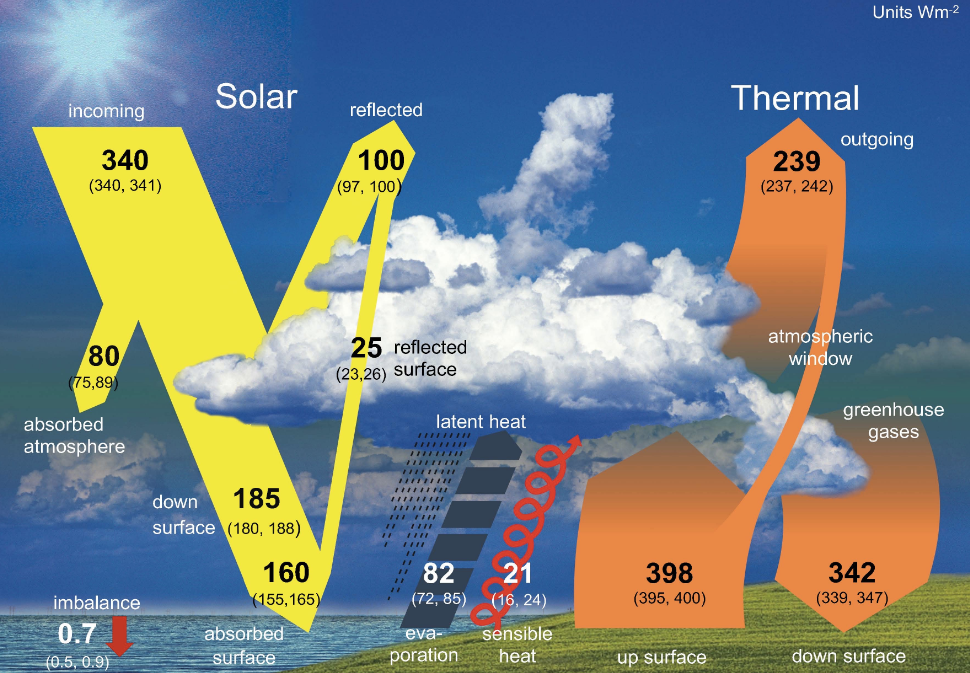
\includegraphics[width=0.1\textwidth]{Secondary/img/Pasted image 20250407181717.png}
% \end{wrapfigure}
\begin{itemize}
    \item 170 PetaWatt (\textit{170 Millionen Kernkraftwerke}) Strahlungsleistung von Sonne / entspricht 340 W/sqm von Sonne
        \begin{itemize}
            \item \textit{70\% absorbiert}
            \item \textit{30\% reflektiert}
        \end{itemize}
    \item Komponenten
        \begin{itemize}
            \item Solare Strahlung
                \begin{itemize}
                    \item Atmosphere Absorptions \& Reflections at Aerosols
                    \item Surface Absorptions \& Reflections
                \end{itemize}
            \item Thermische Strahlung
                \begin{itemize}
                    \item Greenhouse Gases
                    \item Und Andere Effekte
                \end{itemize}
            \item Latente Wärme in Wasserkreislauf
                \begin{itemize}
                    \item Evaporation
                    \item Sensible Heat
                \end{itemize}
        \end{itemize}
    \item \textbf{0.7 W/sqm} = Absorbierte Sonnenenergie (240|70\%) - Emittierte thermische Energie (239)`
    \item 91\% des Energieüberschusses geht in Ozeane \twemoji{ocean}
        \begin{itemize}
            \item Messung durch Netz von Temperatursonden
        \end{itemize}
    \item Regulierung bodennahes Klima durch:
        \begin{itemize}
            \item Strahlungsbilanz an der Erdoberfläche \twemoji{sun_with_face}
            \item Wasserkreislauf
            \item 103 W/sqm have to be compensated by sensible and latent heat fluxes
        \end{itemize}
    \item Menschliche Eingriffe:
        \begin{itemize}
            \item Aerosols <-> Solar
                \begin{itemize}
                    \item Schwefel, Russ, ...
                    \item Temperatur-Abnahme (Decrease > Increase)
                \end{itemize}
            \item GHGs <-> Thermal
                \begin{itemize}
                    \item Temperatur-Zunahme
                \end{itemize}
            \item Landnutzungsänderungen (Albedo) \twemoji{poop}
        \end{itemize}
    \item Messung der Energieflüsse:
        \begin{itemize}
            \item Outgoing mit \textbf{Satelliten}
            \item Incoming mit \textbf{Strahlungsmessstationen am Boden}
        \end{itemize}
\end{itemize}

\subsection{Praktische Anwendung: Solarenergie}
\begin{itemize}
    \item Starke Zunahme der Nutzung von Photovoltaik \twemoji{sunflower}
    \begin{center}
        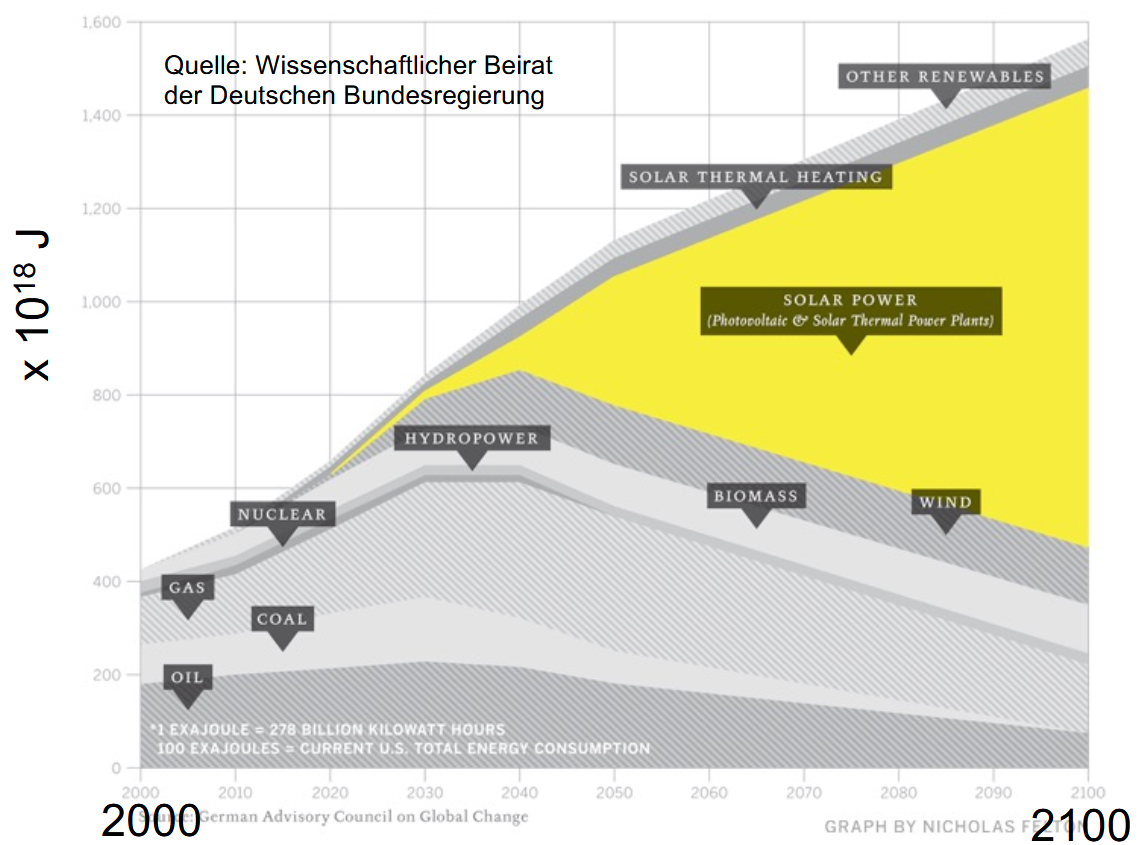
\includegraphics[width=0.12\textwidth]{Secondary/img/Pasted image 20250407180632.png}
    \end{center}
\end{itemize}

\subsection{Solar Output \& Satellite Replacement Issues}
\begin{wrapfigure}{r}{0.125\textwidth}
    \centering
    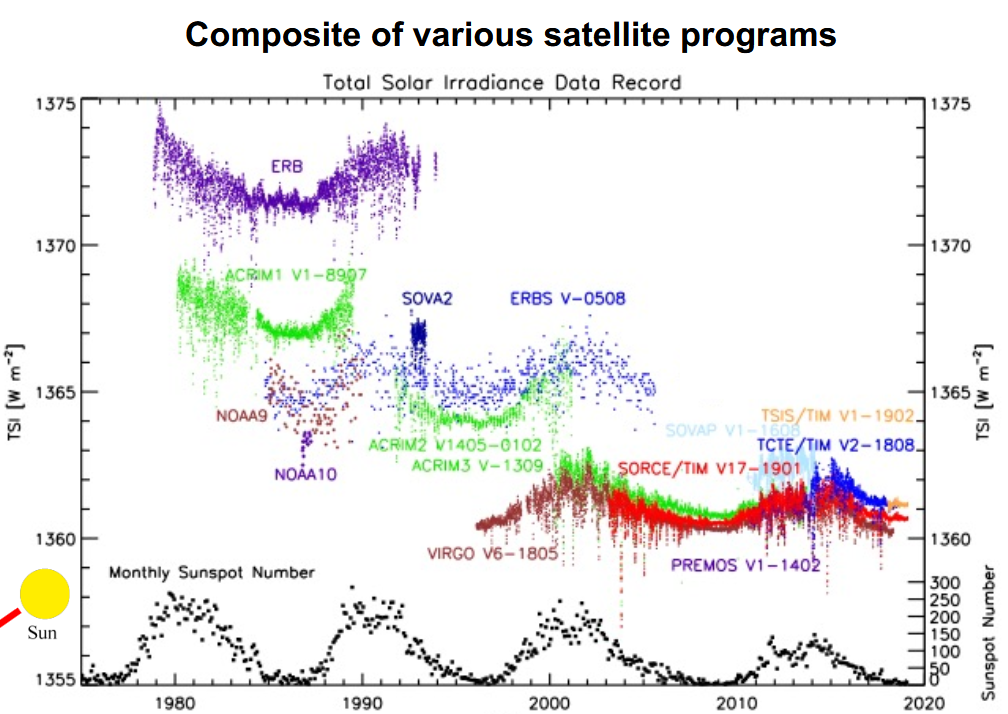
\includegraphics[width=0.12\textwidth]{Secondary/img/Pasted image 20250407180714.png}
\end{wrapfigure}
\begin{itemize}
    \item Difficult to \textbf{unify measurements} from various satellite programs
    \item Facular Brightening overcompensates Sunspot Darkening -> \textbf{more sunspots - more radiation} (counterintuitive)
\end{itemize}

\subsection{Insolation Calculations (Berechnung Strahlungsflüsse)}
\subsubsection{Solar Zenith Angle $\theta$}
\begin{wrapfigure}{r}{0.125\textwidth}
    \centering
    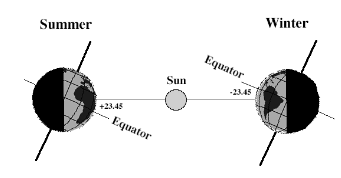
\includegraphics[width=0.12\textwidth]{Secondary/img/Pasted image 20250408115014.png}
\end{wrapfigure}
The Solar zenith angle $\theta$ can be calculated using the following formula:
$$\cos(\theta) = \cos(H) \cos(\phi) \cos(\delta) + \sin(\phi) \sin(\delta)$$
Where:
\begin{itemize}
    \item $H$: Hour angle
        \begin{itemize}
            \item represents the time of day, as a deviation from local noon
            \item calculated based on the seconds until or from local noon
            \item 86400 seconds in 24 hours are corresponding to 360°: $$H = \frac{\text{seconds till or from noon}}{86400} \cdot 360^\circ$$
        \end{itemize}
    \item $\phi$: Latitude
    \item $\delta$: Declination
        \begin{itemize}
            \item represents the calendar day / season
            \item lies between $\pm 23.45^\circ$ due to the Earth's tilt
            \item declination $\delta$ is angle between the sun's rays and the plane of the Earth's equator
        \end{itemize}
\end{itemize}

\subsubsection{Insolation by Location and Time (TOA)}
\begin{wrapfigure}{r}{0.125\textwidth}
    \centering
    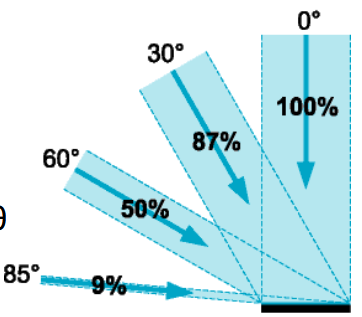
\includegraphics[width=0.08\textwidth]{Secondary/img/Pasted image 20250407180808.png}
\end{wrapfigure}
\begin{itemize}
    \item TOA: Top of Atmosphere
\end{itemize}
The Insolation $I$ can be calculated using the following formula:
$$I = S \cos(\theta)$$
Where:
\begin{itemize}
    \item $I$: Insolation (irradiance) on a horizontal surface
        \begin{itemize}
            \item specific location and time on the globe
            \item neglecting atmospheric effects
        \end{itemize}
    \item $S$: Top of Atmosphere insolation
        \begin{itemize}
            \item on a panel optimally oriented towards the sun
            \item $S$ is dependent on solar activity and the Earth's position in its orbit around the Sun (which is elliptical)
        \end{itemize}
    \item $\theta$: Solar zenith angle at the specified position and time
\end{itemize}

\subsubsection{TOA Hemisphere Season Asymmetry}
\begin{wrapfigure}{r}{0.125\textwidth}
    \centering
    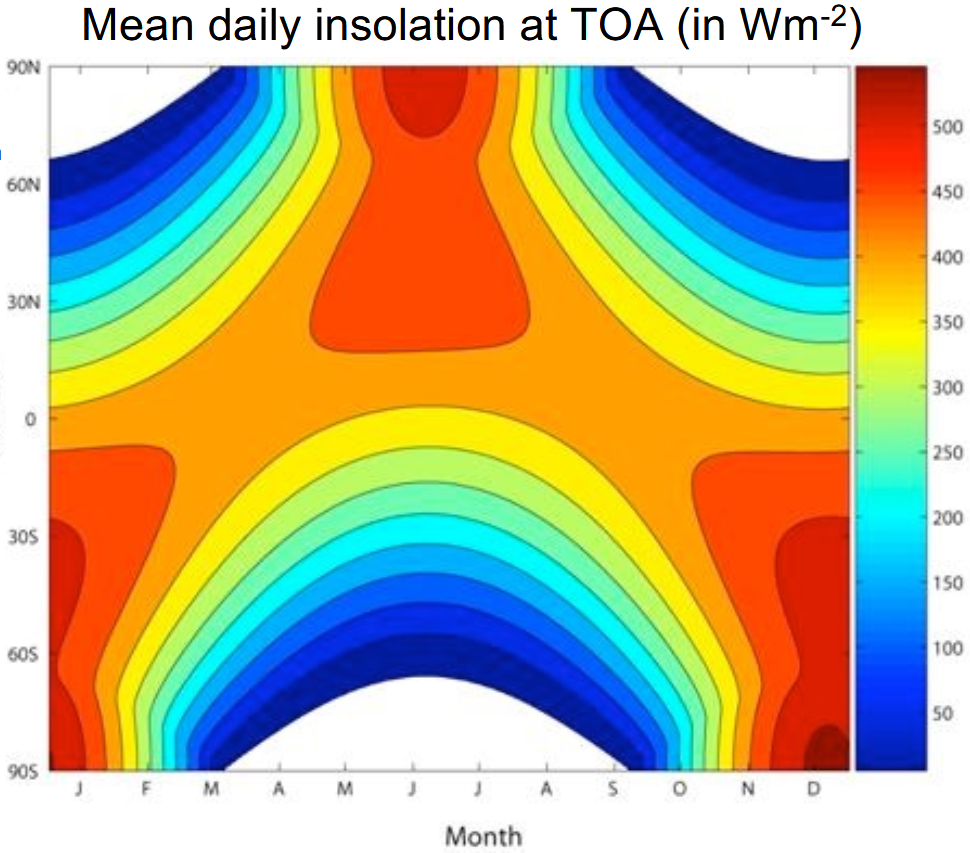
\includegraphics[width=0.08\textwidth]{Secondary/img/Pasted image 20250408112850.png}
\end{wrapfigure}
\begin{itemize}
    \item Süd-Sommer TOA intensiver wegen Perihel
\end{itemize}

\subsubsection{Insolation within the Atmosphere at Depth $h$}
\begin{wrapfigure}{r}{0.125\textwidth}
    \centering
    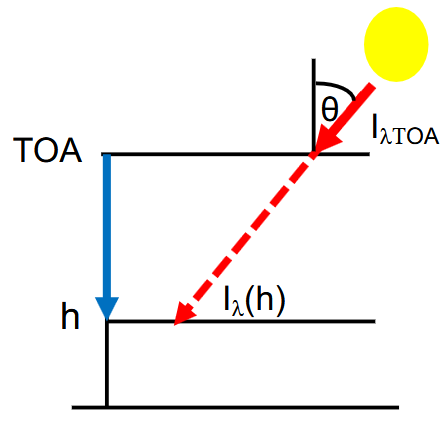
\includegraphics[width=0.12\textwidth]{Secondary/img/Pasted image 20250408114911.png}
\end{wrapfigure}
The insolation $I_\lambda$ at a depth $h$ within the atmosphere, at a specific wavelength $\lambda$, can be calculated using the following formula:
$$I_\lambda(h) = I_{\lambda,TOA} e^{-m\underbrace{\int_{TOA}^hk_\lambda\rho dz}_{\tau_\lambda}}$$
Where:
\begin{itemize}
    \item $I_\lambda(h)$: Insolation at depth $h$ and wavelength $\lambda$
    \item $I_{\lambda,TOA}$: Insolation at the Top of Atmosphere (TOA) and wavelength $\lambda$
        \begin{itemize}
            \item $I_{\lambda,TOA} = S_\lambda \cos(\theta)$
        \end{itemize}
    \item $m$: Optical mass
        \begin{itemize}
            \item $m = \frac{1}{\cos(\theta)}$
            \item accounts for the expansion of optical depth due to the slant path of sunlight through the atmosphere
        \end{itemize}
    \item $\tau_\lambda$: Optical depth at wavelength $\lambda$
        \begin{itemize}
            \item $k_\lambda$: Extinction coefficient at wavelength $\lambda$.
                \begin{itemize}
                    \item $k_\lambda = k_{\lambda,abs} + k_{\lambda,scatt}$
                    \item $k_{\lambda,abs}$: Absorption coefficient at wavelength $\lambda$.
                    \item $k_{\lambda,scatt}$: Scattering coefficient at wavelength $\lambda$.
                \end{itemize}
            \item $\rho$: Density of the atmosphere as a function of z.
        \end{itemize}
\end{itemize}

\subsubsection{Spectrum of solar radiation}
\begin{center}
    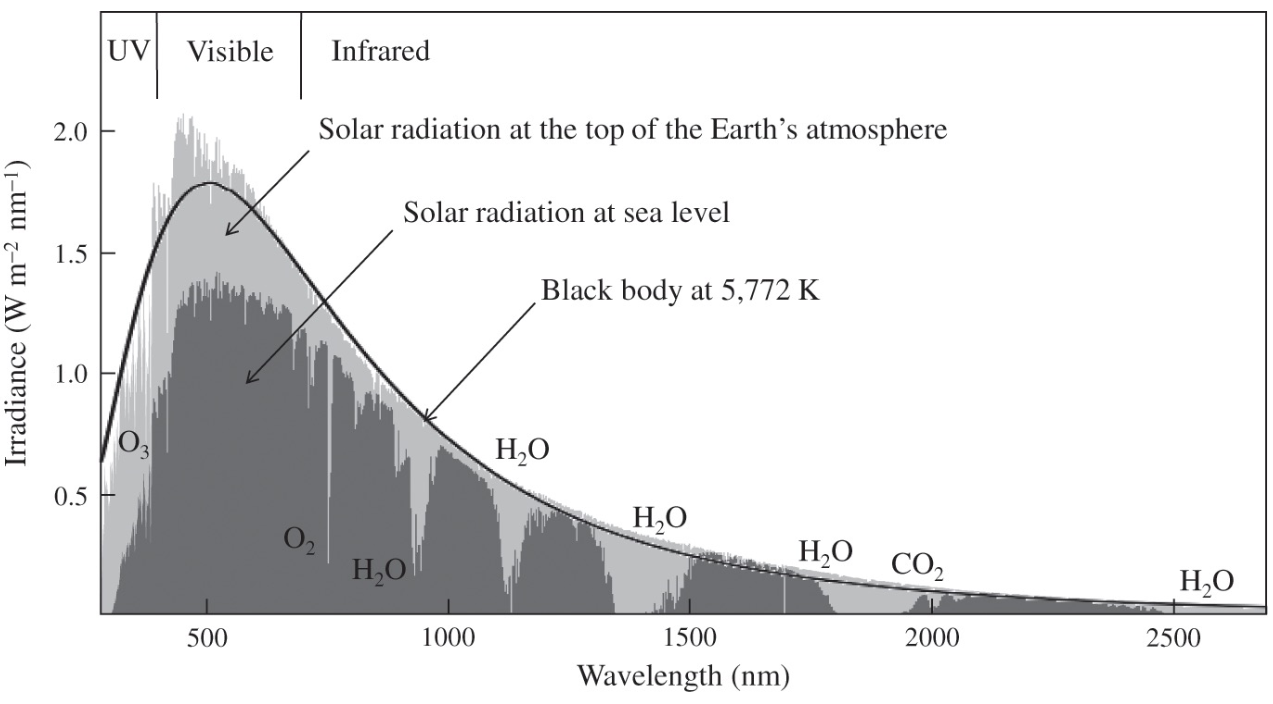
\includegraphics[width=0.12\textwidth]{Secondary/img/Pasted image 20250408120900.png}
\end{center}

\subsection{Human Impacts}
\subsubsection{GHG Temporal Changes}
\begin{itemize}
    \item +2.0 W/sqm/decade - \textit{GHG thermal down surface} Increase at worldwide measurements sites since 1990s
\end{itemize}

\subsubsection{Global Dimming (Aerosols Temporal Changes)}
\begin{itemize}
    \item 10\% \textbf{Global dimming} in 1950s-1980s
        \begin{itemize}
            \item \textbf{Global brightening} since 1980s
        \end{itemize}
    \item Maskierung des Treibhauseffekts
    \item caused by Global Anthropogenic Sulfur Emissions
    \item Both direct and indirect effects reduce the amount of solar radiation reaching the ground
        \begin{itemize}
            \item direct aerosol effects: Scattering \& Absorption
            \item indicect aerosol effects: cloud albedo \& cloud lifetime
        \end{itemize}
    \item 11 - 15\% more PV power for China if it could revert back to the 1960s insolation level
\end{itemize}

\subsubsection{Impact on other CC Aspects}
\begin{itemize}
    \item \textbf{Glacier Area Reduction}:
        \begin{itemize}
            \item -1\% during Dimming
            \item -33\% during Brightening
        \end{itemize}
    \item \textbf{Variations in Rainfall} correlates with Solar Dimming and Brightening
    \item \textbf{Increased plant growth} and \textbf{carbon uptake} during dimming
        \begin{itemize}
            \item More pollution leads to less total and more diffuse solar radiation
            \item Effect of diffuse fraction increase dominates
        \end{itemize}
\end{itemize}

\section{Global Climate Change}
\subsection{Climate Crisis Overview}
\begin{itemize}
    \item The \textbf{global climate crisis} is worsening with \textbf{devastating impacts} like:
        \begin{itemize}
            \item wildfires
            \item heatwaves
            \item floods
            \item significant economic costs
        \end{itemize}
    \item \textbf{Global surface temperatures} have \textbf{increased} significantly above \textbf{pre-industrial} levels
        \begin{itemize}
            \item recent years showing \textit{record warming}
        \end{itemize}
    \item \textbf{Global Impact}
        \begin{itemize}
            \item \textit{Extreme weather events} as a \textit{Major global risk} (Global Risks Perception Survey by World Economic Forum)
            \item including Europe, Canada, and the US
        \end{itemize}
\end{itemize}

\subsection{IPCC and Its Role}
\begin{itemize}
    \item \textbf{Intergovernmental Panel on Climate Change} (IPCC)
        \begin{itemize}
            \item Created in 1988 by the United Nations Environment Programme (UNEP) and the World Meteorological Organization (WMO)
            \item Global organization of governments
            \item Members of the United Nations or WMO
        \end{itemize}
    \item \textbf{Assessment Reports}
        \begin{itemize}
            \item gives scientific evidence on climate change
            \item publishes comprehensive reports on climate change
            \item climate change \textbf{impacts}
            \item potential \textbf{mitigation} strategies
            \item potential \textbf{adaptation} strategies
            \item crucial for international climate negotiations.
        \end{itemize}
\end{itemize}

\subsection{Scientific Evidence}
\begin{itemize}
    \item \textbf{Human activities} are the primary driver of global warming
        \begin{itemize}
            \item burning fossil fuels
            \item land use changes (deforestation, albedo)
        \end{itemize}
    \item \textbf{Observed Changes}
        \begin{itemize}
            \item Some extreme events unlikely without human influence
        \end{itemize}
\end{itemize}

\subsection{Future Projections}
\begin{itemize}
    \item Continued CO2 emissions will lead to:
        \begin{itemize}
            \item \textbf{Further Global Warming}
            \item \textbf{Increasing Extreme Events}: frequency and intensity
        \end{itemize}
    \item \textbf{Emission Scenarios}: Only certain societal scenarios align with 1.5°C goal from Paris Agreement
        \begin{itemize}
            \item Limiting global warming to \textbf{1.5°C} compared to \textbf{2°C} can help avoid significant additional risks and impacts
        \end{itemize}
\end{itemize}

\subsection{Mitigation Strategies}
\begin{itemize}
    \item \textbf{Net-Zero CO2 Emissions} requires:
        \begin{itemize}
            \item drastic reductions in fossil fuel use
            \item increasing renewable energy
            \item implementing carbon capture and storage
        \end{itemize}
\end{itemize}

\subsection{Health and Economic Impacts}
\begin{itemize}
    \item \textbf{Health}:
        \begin{itemize}
            \item Heat-related mortality and other health issues by Climate Change
            \item Improved air quality and public health by reducing emissions
        \end{itemize}
    \item \textbf{Economic Costs}
        \begin{itemize}
            \item Significant economic impacts by Climate Change
            \item Avoiding damage to infrastructure
            \item Avoiding disruptions to supply chains
        \end{itemize}
\end{itemize}

\subsection{Positive Outlook \& Conclusion}
\begin{itemize}
    \item There are \textbf{feasible solutions for decarbonization} existing and relatively inexpensive
        \begin{itemize}
            \item some progress is being made
            \item immediate and substantial action is needed to stabilize global warming at about 1.5°C and meet climate goals
        \end{itemize}
\end{itemize}

\section{Paleoclimate}
\section{Global Water Cycle}
\section{Biomes \& Land-Climate}
\section{Detection and Attribution of Trends \& Extreme Events}
\end{multicols*}
\end{document}